\section{Atividades}

\subsection{Estabelecer Tema de Investimento}

  \textbf{Descrição}: Essa atividade consiste na definição do tema de investimento a partir do \textit{Workshop} de Requisitos realizado.\\

  \textbf{Tarefas}:

  \begin{itemize}
  
    \item \indent \textit{Fazer Análise Documental}: Analisar documentos da empresa e o modelo de negócios produzido pela equipe de Modelagem.
   
   \item \indent \textit{Fazer Workshop de Requisitos}: Reunião com o cliente e o time para levantar requisitos de mais alto nível. Consiste
   em uma técnica de elicitação definida no Capítulo \ref{tecnicas}.

   \item \indent \textit{Validar Tema de Investimento}: Escrever o tema de investimento e confirmar com o cliente se
   o Tema de Investimento estabelecido está correto.
  \end{itemize}

  \textbf{Participantes}: \textit{Product Manager}, \textit{Scrum Master}, Time \\

  \textbf{Entrada}: Modelo de negócio \\

  \textbf{Saída}: Tema de Investimento Validado\\

\subsection{Levantar Épicos}
  \textbf{Descrição}: Essa atividade consiste no levantamento dos épicos com o \textit{Product Manager} através do  \textit{Workshop} de Requisitos. \\

  \textbf{Tarefas}:

  \begin{itemize}
   \item \indent \textit{Fazer Workshop de Requisitos}: Reunião com o cliente e o time para levantar requisitos de mais alto nível. Consiste
   em uma técnica de elicitação definida no Capítulo \ref{tecnicas}.

   \item \indent \textit{Escrever Épicos}: A partir das anotações feitas no \textit{Workshop},
   escrever os épicos no \textit{Backlog} do Programa.
   
   \item \indent \textit{Manter Rastreabilidade}: Registrar na ferramenta cada épico como derivado do tema de investimento.

  \end{itemize}

  \textbf{Participantes}: \textit{Product Manager}, \textit{Scrum Master}, Time \\

  \textbf{Entrada}: Anotações do \textit{Workshop} \\

  \textbf{Saída}: Épicos Validados - \textit{Backlog} do Programa\\

\subsection{Fazer reunião de validação dos épicos}
  \textbf{Descrição}: Essa atividade consiste na apresentação dos épicos especificados para o \textit{Product Manager}, de modo a validar se os épicos
  especificados estão corretos e correspondem ao esperado. \\

  \textbf{Tarefas}:

  \begin{itemize}
    \item \indent \textit{Validar Épicos}: Confirmar em reunião com o cliente se os épicos estabelecidos estão corretos.

   \item \indent \textit{Escrever Épicos}: Se houver alguma mudança solicitada pelo cliente, escrever os épicos
   refinados no \textit{Backlog} do Programa.
  \end{itemize}

  \textbf{Participantes}: \textit{Product Manager}, \textit{Scrum Master}, Time \\

  \textbf{Entrada}: \textit{Backlog} do Programa (Épicos) \\

  \textbf{Saída}:  \textit{Backlog} do Programa (Épicos) \\

\subsection{Levantar \textit{Features}}
\textbf{Descrição}: Essa atividade consiste em listar as \textit{Features}, a partir dos épicos ,
que são as tarefas ou os “serviços” que o sistema deve fornecer para atender as necessidades das partes interessadas.
Deve-se observar se as \textit{features} condizem com ou traduzem de forma clara os Épicos
definidos previamente, e se através delas é possível escrever as Histórias de Usuário.\\

\textbf{Tarefas}:

  \begin{itemize}
   \item \indent \textit{Listagem de \textit{Features}}:  Listar \textit{Features} a partir dos Épicos de Portfólio ou a partir de outras \textit{Features}.

   \item \indent \textit{Adição e Edição de \textit{Features}}: Adicionar novas \textit{Features} ou modificar as \textit{Features} já levantas de acordo com as mudanças sugeridas na Reunião de Validação.

   \item \indent \textit{Manter Rastreabilidade}: Registrar na ferramenta de qual épico é cada \textit{Feature}.
   \end{itemize}

\textbf{Participantes}: \textit{Product Manager}, \textit{Scrum Master}, Time \\

\textbf{Entrada}: \textit{Backlog} do Programa (Épicos) \\

\textbf{Saída}:  \textit{Features} Validadas - \textit{Backlog} do Programa  \\

\subsection{Fazer reunião de validação das \textit{features}}
  \textbf{Descrição}: Essa atividade consiste na apresentação das \textit{features} especificadas para o \textit{Product Manager}, de modo a validar se
  estão corretos e correspondem ao esperado.  \\

  \textbf{Tarefas}:
  \begin{itemize}
   \item \indent \textit{Listagem de \textit{Features}}: Listar as \textit{Features} elicitadas e detalhadas até o momento;

   \item \indent \textit{Comparação \textit{Features}-Épicos}: Comparar as \textit{Features} e os Épicos, validando se as \textit{Features} expressam as iniciativas contidas nos Épicos;

   \item \indent \textit{Corrigir Possíveis Falhas}: Identificar equívocos no levantamento ou elicitação das \textit{Features} e propor mudanças.
  \end{itemize}

  \textbf{Participantes}: \textit{Product Manager}, \textit{Scrum Master}, Time \\

  \textbf{Entrada}: \textit{Backlog} do Programa (\textit{Features})\\

  \textbf{Saída}:   \textit{Backlog} do Programa (\textit{Features})\\

\subsection{Identificar Requisitos Não Funcionais}
  \textbf{Descrição}: Nesta atividade são identificados e descritos os requisitos não funcionais do sistema e são armazenados no \textit{Backlog} do Programa.  \\

  \textbf{Tarefas}:
  \begin{itemize}
   \item \indent \textit{Identificação de Requisitos não Funcionais}: Identificar e descrever os requisitos não funcionais

   \item \indent \textit{Armazenamento no \textit{Backlog}}: Armazenar no \textit{Backlog} do Programa
  \end{itemize}

  \textbf{Participantes}: \textit{Product Manager}, \textit{Scrum Master}, Time \\

  \textbf{Entrada}:  Necessidade de conhecer as restrições tecnológicas impostas\\

  \textbf{Saída}:  Requisitos Não Funcionais - \textit{Backlog} do Programa\\

\subsection{Construir Visão}
  \textbf{Descrição}: Nesta atividade, deve-se compilar as \textit{Features}, com os requisitos não funcionais, incluindo elementos
  regulatórios ou outros padrões de conformidade, e qualquer restrição de design. A partir disso, é possível descrever um panorama da solução a
  ser desenvolvida, refletindo as necessidades das partes interessadas e os recursos propostos para atender essas necessidades. \\

  \textbf{Tarefas}:
  \begin{itemize}
   \item \indent \textit{Reunir Artefatos}: Reunir \textit{Features}, Requisitos não Funcionais, restrições e padrões.

   \item \indent \textit{Sintetizar e Integrar}: Sintetizar todas as entrada, integrando-as em uma visão holística (global) e coesa do projeto.

   \item \indent \textit{Validar o Visão}: Validar junto ao PM a visão estabelecida.

   \item \indent \textit{Planejamento do \textit{RoadMap}}: Planejar o \textit{RoadMap} de entregas das \textit{Features}.
  \end{itemize}

  \textbf{Participantes}: \textit{Product Manager}, \textit{Scrum Master}, Time \\

  \textbf{Entrada}: \textit{Backlog} do Programa \\

  \textbf{Saída}:  Visão Geral do Sistema - Documento de Visão\\

\subsection{Construir \textit{Roadmap}}
  \textbf{Descrição}: A partir da Visão, deve-se elaborar uma espécie de roteiro, que situa e comunica a equipe e o programa em relação ao
  alinhamento dos objetivos de negócios, e fornece visibilidade das entregas ao longo de um cronograma de curto prazo.
  Esse roteiro divide as \textit{features} nas \textit{Releases}. \\

  \textbf{Tarefas}:
  \begin{itemize}
   \item \indent \textit{Reunir Documento de Visão}: Reunir o documento de visão

   \item \indent \textit{Definir Prioridades}: Priorizar \textit{Features} no \textit{Backlog} do programa.

   \item \indent \textit{Alocamento de \textit{Features}}: Alocar \textit{Features} em \textit{Releases}.

   \item \indent \textit{Validar}: Validar com o PM o \textit{Roadmap} construído.
  \end{itemize}

  \textbf{Participantes}: \textit{Product Manager}, \textit{Scrum Master}, Time \\

  \textbf{Entrada}: Documento de Visão \\

  \textbf{Saída}:  \textit{Features} alocadas em \textit{Releases} - \textit{Roadmap}\\

  \subsection{Escrever histórias}
  \textbf{Descrição}: Essa atividade consiste na escrita das histórias em um nível macro, derivadas das \textit{features}, para composição do \textit{Backlog} do Time. \\

  \textbf{Tarefas}:
  \begin{itemize}
   \item \indent \textit{Identificar}: Identificar \textit{features};

   \item \indent \textit{Analisar}: Analisar o nível de prioridade das \textit{features};

   \item \indent \textit{Alocar}: Alocar \textit{features} nas iteração;

   \item \indent \textit{Instruir}: Auxílio do Scrum Master ao Product Manager a fim de ensinamento; de técnicas de escritas de histórias de usuário;

   \item \indent \textit{Escrever}: Escrever histórias;

   \item \indent \textit{Armazenamento}: Armazenar histórias no \textit{Backlog} do time.
   
   \item \indent \textit{Manter Rastreabilidade}: Registrar na ferramenta de qual \textit{Feature} é cada história.

  \end{itemize}

  \textbf{Participantes}: \textit{Product Manager}, \textit{Scrum Master}, Time\\

  \textbf{Entrada}: \textit{Backlog} do Programa \\

  \textbf{Saída}:   Histórias escritas - \textit{Backlog} do Time \\

\subsection{Planejar \textit{Release}}
  \textbf{Descrição}: Essa atividade consiste na priorização das \textit{features} em iterações para a \textit{Release}. \\

  \textbf{Tarefas}:
  \begin{itemize}
   \item \indent \textit{Reunir \textit{Features}}: Reunir \textit{features} envolvidas na \textit{Release};

   \item \indent \textit{Estudar as \textit{Features}}: Estudar as \textit{features} para melhor entendimento de cada uma;

   \item \indent \textit{Definir Indicador de Complexidade}: Definir um identificador para saber quais demandam mais trabalho (horas de serviço);

   \item \indent \textit{Ordenar}: A partir dos resultados obtidos via análise, ordenar das que mostraram maiores métricas de esforço, até as menores, de modo que as mais difíceis sejam executadas o quanto antes.
  \end{itemize}

  \textbf{Participantes}: \textit{Product Manager}, \textit{Scrum Master}, Time\\

  \textbf{Entrada}: \textit{Backlog} do Programa \\

  \textbf{Saída}:  \textit{Backlog} do Programa \\

\subsection{Gerenciar mudanças no Programa}
  \textbf{Descrição}: Essa atividade consiste na gerência de mudanças no nível de programa, como o surgimento de novas 
  \textit{features}, novos épicos e novas histórias. Para cada um dos níveis de abstração requisitos essa atividade gera saída
  para uma atividade diferente.\\

  \textbf{Tarefas}:
  \begin{itemize}
   \item \indent \textit{Verificar o surgimento de novos requisitos}: Analisar se novos requisitos surgiram;

   \item \indent \textit{Analisar impacto da mudança}: Analisar o impacto e a relevância da mudança no projeto e decidir se será considerada
   ou descartada;

   \item \indent \textit{Registrar novos requisitos}: Registrar novos requisitos, se forem épicos realizar as atividades: Levantar Épicos e 
   Fazer reunião de validação dos épicos. Se forem \textit{features} realizar as atividades: Levantar Épicos e \textit{Features}  
   Fazer reunião de validação dos \textit{features} e se forem histórias realizar a atividade de Escrever histórias.
  
  \end{itemize}

  \textbf{Participantes}: Time\\

  \textbf{Entrada}: \textit{Backlog} do Programa e do Time \\

  \textbf{Saída}:  \textit{Backlog} do Programa e do Time \\

\begin{figure}[!htb]
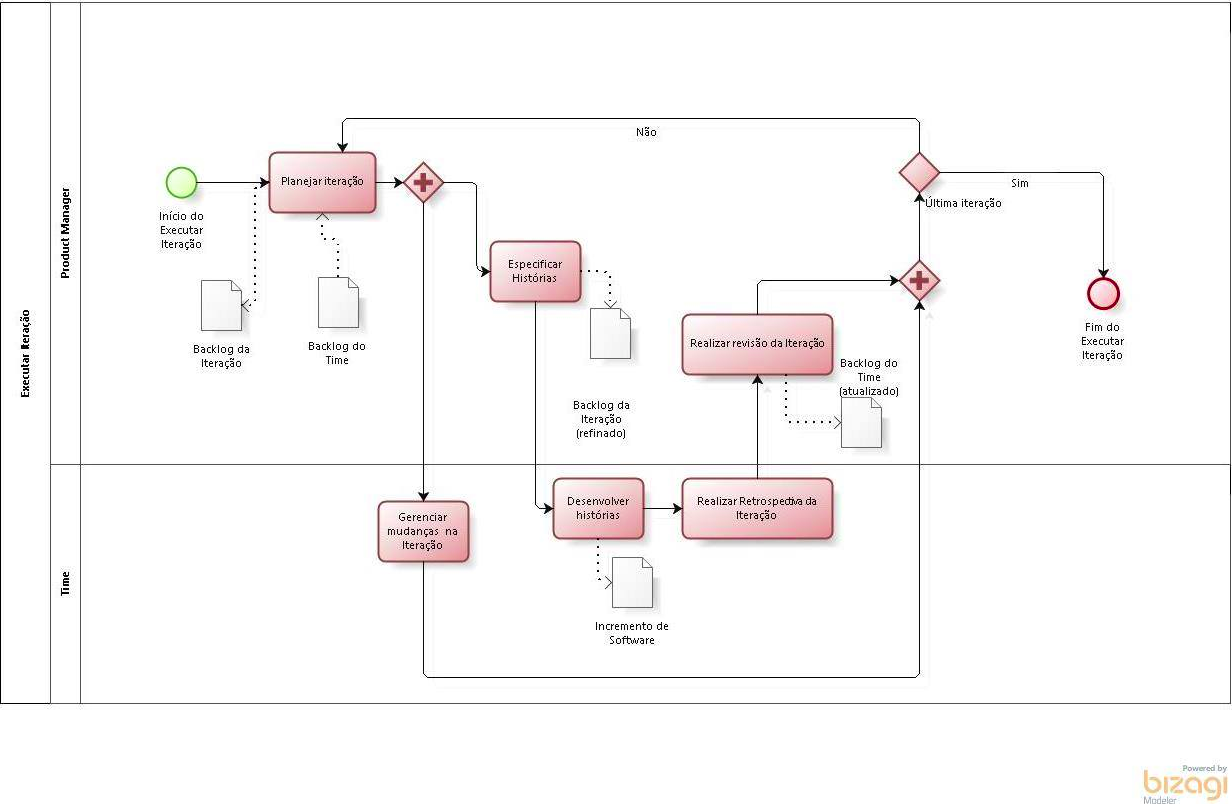
\includegraphics[scale=0.5]{figuras/iteracao2.png}
\caption{Suprocesso Executar Iteração - Versão 2}
\label{fig:iteracao}
\end{figure}

A partir do Subprocesso da Figura \ref{fig:iteracao} o processo contém as seguintes atividades.

\subsection{Realizar reunião de planejamento da Iteração}
  \textbf{Descrição}: Essa atividade consiste no planejamento da iteração através da alocação das histórias definidas no \textit{Backlog} do Time para o \textit{Backlog} da iteração. \\

  \textbf{Tarefas}:
  \begin{itemize}
   \item \indent \textit{Alocação das Histórias}: Alocação das histórias no \textit{Backlog} da iteração

   \item \indent \textit{Armazenamento de Artefatos}: Armazenar no \textit{Backlog} de Iteração
  \end{itemize}

  \textbf{Participantes}: \textit{Product Manager}, \textit{Scrum Master}, Time\\

  \textbf{Entrada}: \textit{Backlog} do Time \\

  \textbf{Saída}:  \textit{Backlog} da Iteração\\

\subsection{Especificar histórias}
  \textbf{Descrição}: Essa atividade consiste na escrita mais detalhada das histórias que irão compor a
iteração. \\

  \textbf{Tarefas}:
  \begin{itemize}
   \item \indent \textit{Detalhamento das Histórias}: Detalhar histórias da iteração
   
   \item \indent \textit{Testes de aceitação}: Escrever testes de aceitação das histórias da iteração

   \item \indent \textit{Armazenamento de Artefatos}: Armazenar no \textit{Backlog} de Iteração

   \item \indent \textit{Atualizar}: Atualizar \textit{Backlog} do Time
  \end{itemize}

  \textbf{Participantes}: \textit{Product Manager}, \textit{Scrum Master}, Time\\

  \textbf{Entrada}: \textit{Backlog} da Iteração \\

  \textbf{Saída}:   \textit{Backlog} da Iteração\\

\subsection{Desenvolver histórias}
  \textbf{Descrição}: Essa atividade consiste no desenvolvimento e teste das histórias contidas no \textit{Backlog} da Iteração. Tem uma duração de 1 semana. \\

  \textbf{Tarefas}:

  \begin{itemize}
    \item \indent \textit{Desenvolver Histórias}: Implementar as histórias contidas no \textit{Backlog} da Iteração.

   \item \indent \textit{Testar Histórias}: Realizar testes unitários do código implementado na iteração e testes funcionais
   com base nos testes de aceitação.
  \end{itemize}

  \textbf{Participantes}: Time\\

  \textbf{Entrada}: \textit{Backlog} da Iteração \\

  \textbf{Saída}:   Incremento de Software\\

\subsection{Fazer reunião de revisão e retrospectiva da Iteração}
  \textbf{Descrição}: Essa atividade consiste na validação das histórias implementadas através da execução dos testes de aceitação. \\

  \textbf{Tarefas}:
  \begin{itemize}
   \item \indent \textit{Análise de Artefatos}: Analisar artefatos gerados na iteração;

   \item \indent \textit{Avaliar Pontos Positivos}: Definir pontos que ocorreram bem;

   \item \indent \textit{Definir Pontos de Melhoria}: Definir pontos que necessitam de melhoria;

   \item \indent \textit{Definir Novas Metas}: Definir novas metas de melhoria a serem alcançadas na nova iteração.
   
   \item \indent \textit{Atualizar o \textit{Backlog}}: Atualizar o \textit{Backlog} do Time.
  \end{itemize}

  \textbf{Participantes}: \textit{Product Manager}, Time\\

  \textbf{Entrada}: Incremento de Software \\

  \textbf{Saída}:   \textit{Backlog} do Time \\

\subsection{Gerenciar mudanças na Iteração}
  \textbf{Descrição}: Essa atividade consiste na gerência de mudanças no nível de time, como o surgimento ou alocação de novas histórias.\\

  \textbf{Tarefas}:
  \begin{itemize}
   \item \indent \textit{Verificar o surgimento de novos histórias}: Analisar se novas histórias surgiram;

   \item \indent \textit{Verificar a necessidade de realocar histórias}: Analisar se será necessário realocar histórias em outra iteração;
   
   \item \indent \textit{Analisar impacto da mudança}: Analisar o impacto e a relevância da mudança na iteração e decidir se será considerada
   ou descartada;

   \item \indent \textit{Registrar novas histórias}: Registrar novas histórias e realizar a atividade de Escrever histórias.

   \item \indent \textit{Realocar histórias}: Realocar as histórias em outra iteração.
  \end{itemize}

  \textbf{Participantes}: Time\\

  \textbf{Entrada}: \textit{Backlog} do Time e da Iteração\\

  \textbf{Saída}:  \textit{Backlog} do Time e da Iteração\\